\documentclass[compress]{beamer}
\usepackage{ifthen,verbatim}

\newcommand{\isnote}{}
\xdefinecolor{lightyellow}{rgb}{1.,1.,0.25}
\xdefinecolor{darkblue}{rgb}{0.1,0.1,0.7}

%% Uncomment this to get annotations
%% \def\notes{\addtocounter{page}{-1}
%%            \renewcommand{\isnote}{*}
%% 	   \beamertemplateshadingbackground{lightyellow}{white}
%%            \begin{frame}
%%            \frametitle{Notes for the previous page (page \insertpagenumber)}
%%            \itemize}
%% \def\endnotes{\enditemize
%% 	      \end{frame}
%%               \beamertemplateshadingbackground{white}{white}
%%               \renewcommand{\isnote}{}}

%% Uncomment this to not get annotations
\def\notes{\comment}
\def\endnotes{\endcomment}

\setbeamertemplate{navigation symbols}{}
\setbeamertemplate{headline}{\mbox{ } \hfill
\begin{minipage}{5.5 cm}
\vspace{-0.75 cm} \small
\end{minipage} \hfill
\begin{minipage}{4.5 cm}
\vspace{-0.75 cm} \small
\begin{flushright}
\ifthenelse{\equal{\insertpagenumber}{1}}{}{Jim Pivarski \hspace{0.2 cm} \insertpagenumber\isnote/\pageref{numpages}}
\end{flushright}
\end{minipage}\mbox{\hspace{0.2 cm}}\includegraphics[height=1 cm]{../cmslogo} \hspace{0.1 cm} \includegraphics[height=1 cm]{../tamulogo} \hspace{0.01 cm} \vspace{-1.05 cm}}

\newcommand{\s}[1]{{\mbox{\scriptsize #1}}}

\begin{document}
\begin{frame}
\vfill
\begin{center}
\textcolor{darkblue}{\Large Search for Dimuon Resonances in ``Lepton Jets''}

\vfill
\begin{columns}
\column{0.3\linewidth}
\begin{center}
\large
\textcolor{darkblue}{\it Jim Pivarski}

Alexei Safonov

Aysen Tatarinov

\vspace{0.5 cm}
\scriptsize
{\it Texas A\&M University}

\vspace{0.5 cm}
\normalsize
8 March, 2011
\end{center}

\column{0.35\linewidth}
\includegraphics[width=\linewidth]{eventdisplay_3d.png}
\end{columns}

\end{center}
\end{frame}

%% \begin{notes}
%% \item This is the annotated version of my talk.
%% \item If you want the version that I am presenting, download the one
%% labeled ``slides'' on Indico (or just ignore these yellow pages).
%% \item The annotated version is provided for extra detail and a written
%% record of comments that I intend to make orally.
%% \item Yellow notes refer to the content on the {\it previous} page.
%% \item All other slides are identical for the two versions.
%% \end{notes}

\small

\section*{Introduction and method}

%% \begin{frame}
%% \frametitle{Outline}
%% \begin{itemize}\setlength{\itemsep}{0.75 cm}
%% \item 
%% \end{itemize}
%% %% \hspace{-0.83 cm} \textcolor{darkblue}{\Large Outline2}
%% \end{frame}

\begin{frame}
\frametitle{Sketch of the basic goal}
\includegraphics[width=\linewidth]{basic_picture.pdf}

\vspace{0.5 cm}
\begin{itemize}
\item Hidden-valley picture: predicts new low-mass, high-momentum particles decaying to Standard Model pairs like $\mu\mu$
\item We want to maximize our sensitivity to ``something like this''
\begin{itemize}
\item strike a balance between accepting theoretical guidance and producing a general result
\end{itemize}
\end{itemize}
\end{frame}

\begin{frame}
\frametitle{Motivation from PAMELA result}
\includegraphics[width=\linewidth]{basic_picture2.pdf}

\vspace{0.5 cm}
\begin{itemize}
\item Sub-class motivated by PAMELA positron excess
\begin{itemize}
\item the ``something light'' is a long-range force between WIMPs
\item unobserved antiproton excess is kinematically forbidden
\end{itemize}
\item Would appear in $pp$ collisions as high-$\vec{p}$, low-mass $Z/\gamma$-like objects
\end{itemize}
\end{frame}

\begin{frame}
\frametitle{Overview of the method (1/5)}

\renewcommand{\arraystretch}{1.7}
\begin{tabular}{p{0.6\linewidth} | p{0.35\linewidth}}
Theoretical guidance & Experimental method \\\hline

couplings within the hidden sector (dark matter, NMSSM Higgs, etc.) are stronger than couplings to the Standard Model, so only the lightest hidden particle ($m_1$) decays visibly & search for one new low-mass particle \\

\centering \includegraphics[width=0.8\linewidth]{basic_picture4.pdf} & \\

assume no fine splittings ($M_2 - M_1 \gg m$), such that some low-mass $m_i$ is on-shell & search for $m_1$ or $m_2$ resonance peak \\
\end{tabular}
\end{frame}

\begin{frame}
\frametitle{Overview of the method (2/5)}

\renewcommand{\arraystretch}{1.7}
\begin{tabular}{p{0.6\linewidth} | p{0.35\linewidth}}
Theoretical guidance & Experimental method \\\hline

several $m_1$ may appear per event, and their decay products may overlap

cascades of low-mass particles would be collimated by a high-momentum boost & identify well-separated groups with a clustering algorithm \\

\centering \includegraphics[width=0.55\linewidth]{basic_picture5.pdf} & \\

$\mathcal{B}(m_1 \to \mu\mu)$ is likely to be high (DY-like if $m_1$ mixes with $\gamma$, $\sim$20\% if Higgs-like, \ldots)

\vspace{0.2 cm}
but non-$\mu\mu$ decays would also happen, so $m_1 \to \mu\mu$ could overlap electrons/pions & look for dimuons, but neither require nor exclude other particles (e.g.\ do not apply an isolation cut) \\
\end{tabular}
\end{frame}

\begin{frame}
\frametitle{Overview of the method (3/5)}

\renewcommand{\arraystretch}{1.7}
\begin{tabular}{p{0.35\linewidth} | p{0.6\linewidth}}
Theoretical guidance & Experimental method \\\hline

narrow groups of four or more muons come from cascades like $m_2 \to m_1 m_1$ with both $m_1 \to \mu\mu$ & resolve combinatorics within each group by finding the most consistent combination of dimuon masses ($a$ and $b$ such that $m_a \approx m_b$)

\vspace{0.3 cm}
\centering \includegraphics[width=0.8\linewidth]{four-two-muon-mass.pdf}

\vspace{-0.75 cm}
\end{tabular}
\end{frame}

\begin{frame}
\frametitle{Overview of the method (4/5)}

\renewcommand{\arraystretch}{1.7}
\begin{tabular}{p{0.4\linewidth} | p{0.55\linewidth}}
Theoretical guidance & Experimental method \\\hline

only the lightest hidden state decays to muon pairs, so only one new mass & in the dimuon mass-dimuon mass plane, signal is a peak on the $m_a \approx m_b$ diagonal, background is diffuse \\

\includegraphics[width=\linewidth]{basic_picture4.pdf} & 
\includegraphics[width=\linewidth]{diagonal.png}

determine signal and background yields from a simultaneous fit, where the ``sideband'' is the non-diagonal part \\

& shape of fit function derived from similar datasets
\end{tabular}
\end{frame}

\begin{frame}
\frametitle{Overview of the method (5/5)}

\renewcommand{\arraystretch}{1.7}
\begin{tabular}{p{0.35\linewidth} | p{0.6\linewidth}}
Theoretical guidance & Experimental method \\\hline

cross-section $\lesssim \mathcal{O}(\mbox{pb})$

\vspace{0.25 cm}
many topologies possible; typically high-momentum and/or high muon multiplicity & design search regions to exclude backgrounds rather than seek any particular topology

\begin{center}
\includegraphics[width=0.8\linewidth]{signal_regions.pdf}
\end{center}

divide momentum and multiplicity space into non-overlapping signal regions, \mbox{excluding low-momentum,} low multiplicity

\vspace{0.25 cm}
(listed on next page)
\end{tabular}
\end{frame}

\begin{frame}
\frametitle{Event selection/signal regions}

\vspace{0.25 cm}
\hfill \mbox{\includegraphics[width=0.37\linewidth]{closeness.pdf}\hspace{-0.6 cm}}

\vspace{-3.5 cm}
\textcolor{darkblue}{All signal events must have:}

\begin{itemize}
\item at least one $p_T > 15$~GeV/$c$, $|\eta| < 0.9$ muon
\item HLT\_Mu15 or equivalent
\item at least one cluster of muons (``mu-jet'')
\end{itemize}

\vspace{0.15 cm}
\textcolor{darkblue}{Specific signal regions:}

\vspace{0.1 cm}
\begin{columns}
\column{0.02\linewidth}
\mbox{ }

\column{0.65\linewidth}
\renewcommand{\arraystretch}{1.3}
\begin{tabular}{c l l}
\hline name & description & min mu-jet $p_T$ \\\hline
$R^1_2$ & high-$p_T$ dimuon & 80~GeV/$c$ \\
$R^1_4$ & four nearby muons & 30~GeV/$c$ \\
$R^2_{22}$ & two separate \mbox{dimuons\hspace{-0.3 cm}} & 20, 10~GeV/$c$ \\
$R^N_{5+}$ & high multiplicity & same as above \\\hline
\end{tabular}

\vspace{0.1 cm}
\hspace{0.2 cm} $R^N_{n_1 \cdots n_N}$ has $N$ mu-jets, $n_i$ muons in mu-jet $i$

\column{0.18\linewidth}
\centering \scriptsize no cuts on the number of isolated muons

\vspace{0.3 cm} $R^1_3$ is not signal

\vspace{0.2 cm} $R^{2+}_{\cdots 3 \cdots}$ is signal
\end{columns}

\vspace{0.45 cm}
\textcolor{darkblue}{Muon cuts:} TrackerMuon $p_T > 5$~GeV/$c$, $|\eta| < 2.4$, arbitrated seg.\ $\ge$ 2, \\
\textcolor{white}{Muon cuts:} tracker hits $\ge$ 8, $\chi^2/N_\s{dof} < 4$
\end{frame}

\begin{frame}
\frametitle{Yields with background PDFs}

Zero events in $R^N_{5+}$, nothing on-diagonal in any 2-D region

\begin{columns}
\column{0.5\linewidth}
\includegraphics[width=\linewidth]{signal_a1_data-bkgpdf2.pdf}

\column{0.5\linewidth}
\includegraphics[width=\linewidth]{model_data_a2_m_inv_w22.pdf}
\end{columns}

\begin{columns}
\column{0.5\linewidth}
\centering \includegraphics[width=0.9\linewidth]{b1_2dpdf.png}

\column{0.5\linewidth}
\centering \includegraphics[width=0.9\linewidth]{a2_2dpdf.png}
\end{columns}
\end{frame}

\begin{frame}
\frametitle{Event displays}

\begin{columns}
\column{0.5\linewidth}
\centering $R^2_{22}$: two separate dimuons

(sample event)

\includegraphics[width=\linewidth]{dimudimu_control_eventdisplay.png}

\column{0.6\linewidth}

\vspace{0.1 cm}
\centering $R^1_4$: four nearby muons

(only event)

\includegraphics[width=\linewidth]{quadmu_control_eventdisplay.png}
\end{columns}
\end{frame}

\begin{frame}
\frametitle{Outline for the rest of this talk}
\begin{itemize}\setlength{\itemsep}{0.5 cm}
\item Muon and trigger selection, efficiency
\item Modeling the signal shape
\item Analysis of background physics
\item Modeling the background shapes
\item Fits and model-independent results
\item Benchmark models and model-dependent results
\end{itemize}
\end{frame}

\section*{Muon selection, trigger selection, and efficiencies}
\begin{frame}
\begin{center}
\Huge \textcolor{blue}{Muon selection, trigger selection, and efficiencies}
\end{center}
\end{frame}

\begin{frame}
\frametitle{Muon reconstruction efficiency}

\vspace{0.15 cm}
\textcolor{darkblue}{StandAloneMuons, and hence GlobalMuons, are inefficient when crossing:}

\vspace{0.15 cm}
\begin{columns}
\column{0.3\linewidth}
\includegraphics[width=\linewidth]{muoneverything.pdf}

\column{0.35\linewidth}
\centering GlobalMuons

\includegraphics[width=\linewidth]{endcap_dphi_bypt_twoGlobalMuons.pdf}

\column{0.35\linewidth}
\centering TrackerMuons

\includegraphics[width=\linewidth]{endcap_dphi_bypt_twoTrackerMuons.pdf}
\end{columns}

\vspace{0.35 cm}
\textcolor{darkblue}{Efficiency of reconstructing {\it dimuon} with TrackerMuons + analysis cuts:}

\begin{columns}
\column{0.8\linewidth}
\mbox{\hspace{1 cm}\includegraphics[width=0.5\linewidth]{pt_mass5cut_twoTrackerMuons.pdf}
\includegraphics[width=0.5\linewidth]{eta_mass5cut_twoTrackerMuons.pdf}\hspace{-5 cm}}

\column{0.15\linewidth}
\scriptsize \centering black: crossing in muon system

\vspace{0.2 cm}
\textcolor{red}{red: not crossing}
\end{columns}
\end{frame}

\begin{frame}
\frametitle{Trigger efficiency}

Trigger efficiencies are strongly dependent on whether muons cross in
the muon system, with the exception of single-muon unisolated barrel
trigger (middle of left plot)

\vspace{0.5 cm}
\begin{columns}
\column{0.3\linewidth}
\centering single-muon (HLT\_Mu15)

\includegraphics[width=\linewidth]{eta_mass5cut_triggerMu15_nosuppressedzero.pdf}

\column{0.3\linewidth}
\centering single-muon isolated (HLT\_IsoMu9)

\includegraphics[width=\linewidth]{eta_mass5cut_triggerIsoMu9.pdf}

\column{0.3\linewidth}
\centering double-muon (HLT\_DoubleMu3)

\includegraphics[width=\linewidth]{eta_mass5cut_triggerDoubleMu3.pdf}

\column{0.15\linewidth}
\scriptsize \centering black: crossing in muon system

\vspace{0.2 cm}
\textcolor{red}{red: not crossing}
\end{columns}

\vspace{0.5 cm}
Accepting endcap-triggered events would introduce a strong efficiency
dependence on dimuon kinematics; therefore, we require at least one
$|\eta| < 0.9$ muon above trigger threshold ($p_T > 15$~GeV/$c$)
\end{frame}

\section*{Modeling the signal shape}
\begin{frame}
\begin{center}
\Huge \textcolor{blue}{Modeling the signal shape}
\end{center}
\end{frame}

\begin{frame}
\frametitle{Resolution from SM resonances}

A hidden-sector particle must, by definition, have a narrow width, so
use narrow Standard Model resonances to determine detector resolution

\vspace{0.25 cm}
\includegraphics[width=0.25\linewidth]{respeak_omega_barrel.pdf}
\includegraphics[width=0.25\linewidth]{respeak_phi_barrel.pdf}
\includegraphics[width=0.25\linewidth]{respeak_jpsi_barrel.pdf}
\includegraphics[width=0.25\linewidth]{respeak_psiprime_barrel.pdf}

\vspace{0.25 cm}

These resonances are on the lowest-$p_T$ edge of our desired range:
determine $p_T$-scaling (and fill in gaps between masses) with
Monte Carlo

\vspace{0.25 cm}
\includegraphics[width=0.5\linewidth]{resolution_barrel.pdf}
\includegraphics[width=0.5\linewidth]{resolution_endcap.pdf}
\end{frame}

\section*{Analysis of background physics}
\begin{frame}
\begin{center}
\Huge \textcolor{blue}{Analysis of background physics}
\end{center}
\end{frame}

\begin{frame}
\frametitle{Physics of dimuon backgrounds}

\begin{columns}
\column{0.5\linewidth}
\only<1>{\includegraphics[width=\linewidth]{support_mass_all.pdf}}\only<2>{\includegraphics[width=\linewidth]{support_mass_all_logy.pdf}}

\column{0.5\linewidth}
Data/MC comparison study to understand all background sources
\begin{itemize}
\item diagnostic tool: $b\bar{b}$ cuts = $Iso > 4.5$~GeV/$c$ or $L_{xy} > \mbox{2 mm\hspace{-1 cm}}$
\item ``low-mass rise'' now understood to be Drell-Yan (though MC is incomplete)
\end{itemize}
\end{columns}

\begin{columns}
\column{0.5\linewidth}
\only<1>{\includegraphics[width=\linewidth]{support_mass_bbbar.pdf}}\only<2>{\includegraphics[width=\linewidth]{support_mass_bbbar_logy.pdf}}

\column{0.5\linewidth}
\only<1>{\includegraphics[width=\linewidth]{support_mass_antibbbar.pdf}}\only<2>{\includegraphics[width=\linewidth]{support_mass_antibbbar_logy.pdf}}
\end{columns}
\end{frame}

\section*{Modeling the background shapes}
\begin{frame}
\begin{center}
\Huge \textcolor{blue}{Modeling the background shapes}
\end{center}
\end{frame}

\begin{frame}
\frametitle{Background shape of $R^1_2$}

Different physics sources contribute to each signal region, so
the background shape templates must be individually constructed

\hfill \mbox{\includegraphics[width=0.50\linewidth]{support_bbbarcut_limits.png}\hspace{-0.75 cm}}

\vspace{-3.8 cm}
\begin{itemize}
\item \textcolor{darkblue}{For $R^1_2$:} note that the prompt and \\ isolated, \textcolor{red}{$b\bar{b}$-like,} \textcolor{violet}{and $J/\psi$} com- \\ ponents all scale as {\scriptsize $\exp(-p_T/10\mbox{ GeV})$} \\ above 40~GeV/$c$

\item Derive shape from high-statistics \\ low-$p_T$ data, test in medium-$p_T$, \\ and use in high-$p_T$ signal search
\end{itemize}

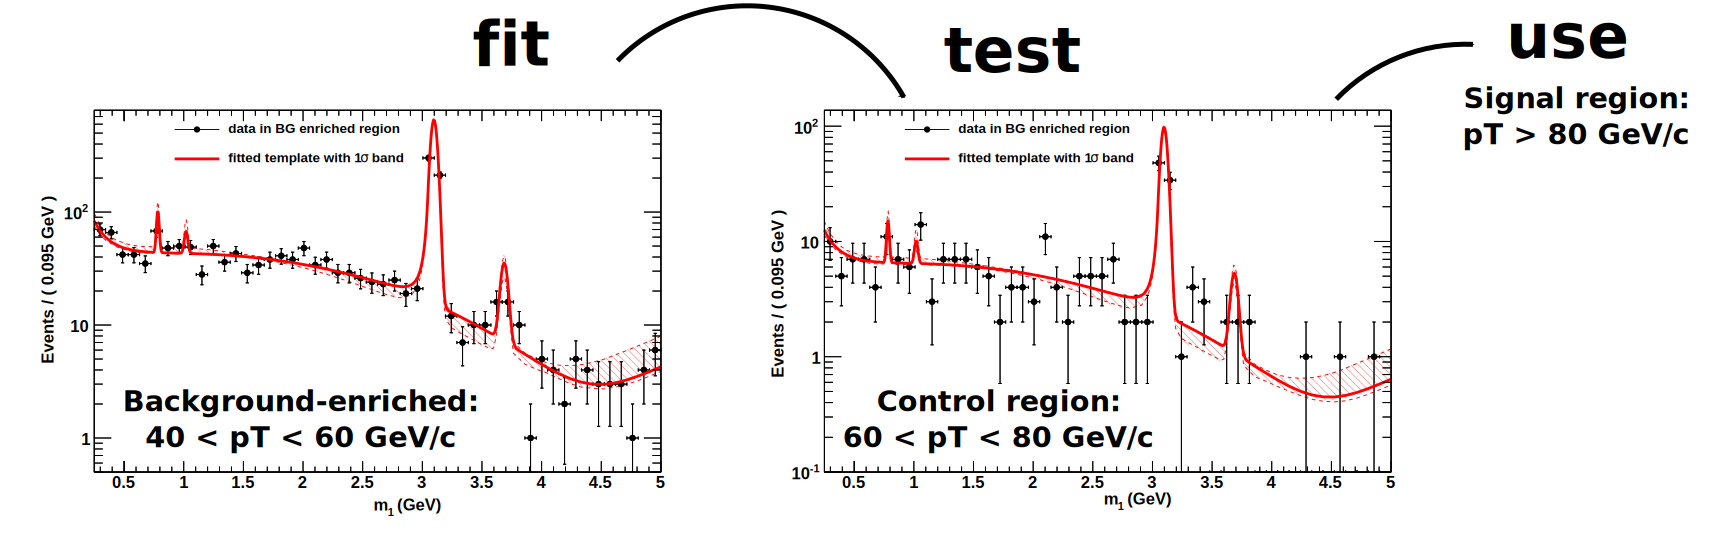
\includegraphics[width=\linewidth]{background_shape_a1.png}
\end{frame}

\begin{frame}
\frametitle{Background shape of $R^1_4$}

\hfill \includegraphics[height=3 cm]{quadmu_control_eventdisplay.png}

\vspace{-3 cm}
\textcolor{darkblue}{For $R^1_4$: four nearby muons}
\begin{itemize}
\item Dominant Standard Model backgrounds: \\ decays-in-flight and misreconstruction (fakes)

\item Simulate fake muons by putting non-muon \\ tracks into mu-jets:
\end{itemize}

\vspace{-0.4 cm}
\renewcommand{\arraystretch}{1.3}
\begin{center}
\begin{tabular}{c c c}
Background-enriched & Control & Signal Region \\\hline
2 muons, 2 tracks & 3 muons, 1 track & 4 muons
\end{tabular}
\end{center}

\vspace{-0.2 cm}
\begin{itemize}
\item Plots of control region with template shape overlaid:
\end{itemize}

\vspace{-0.2 cm}
\mbox{ } \hfill \includegraphics[height=3.5 cm]{a2_control.pdf} \hfill
\includegraphics[height=3.5 cm]{template_control__bkg_model_a2__m_1.pdf} \hfill \mbox{ }
\end{frame}

\begin{frame}
\frametitle{$R^1_4$ four-muon mass shape}

\hfill \includegraphics[height=3 cm]{quadmu_control_eventdisplay.png}

\vspace{-3 cm}
\textcolor{darkblue}{Still $R^1_4$: four nearby muons}

\vspace{0.25 cm}
Considering the case of $m_2 \to m_1 m_1 \to 4\mu$ with \\ $m_1$
off-shell but $m_2$ on-shell, we prepare a template \\ for the four-muon mass

\begin{itemize}
\item background-enriched, control, and signal samples \\ are the same as on the previous page
\item four-muon mass has a two-peak structure: second peak is $J/\psi$
\end{itemize}

\begin{columns}
\column{0.5\linewidth}
\centering background-enriched fit

\includegraphics[width=\linewidth]{template__bkg_model_a2_inv__m_inv.png}

\column{0.5\linewidth}
\centering control sample test

\includegraphics[width=\linewidth]{template_control__bkg_model_a2_inv__m_inv.png}
\end{columns}
\end{frame}

\begin{frame}
\frametitle{Background shape of $R^2_{22}$}

\textcolor{darkblue}{For $R^2_{22}$: two separate dimuons}

\vspace{-0.5 cm}
\hfill \mbox{\includegraphics[height=3.5 cm]{dimudimu_control_eventdisplay.png}\hspace{-0.75 cm}}

\vspace{-3.2 cm}
\begin{itemize}
\item Dominant Standard Model backgrounds: \\ $b\bar{b}$ with both
  $b$-quarks producing $\mu\mu X$ by \\ double-semileptonic decay,
  resonances, etc.
\item Assume that each $b$-quark decays independently \\ and construct
  2-D distribution from Cartesian \\ product of 1-D $b\to\mu\mu X$ distributions
\item Complication: requiring a $p_T > 15$~GeV/$c$ trigger muon
  changes the distribution; need templates for both cases
\end{itemize}

\begin{columns}
\column{0.5\linewidth}
\centering \only<1>{template for dimuon with trigger}\only<2>{control (non-diagonal signal region)}

\only<1>{\includegraphics[width=\linewidth]{template__bg_sh_b1t__m_1_log.png}}
\only<2>{\includegraphics[width=0.75\linewidth]{b1_2dpdf.png}}

\column{0.5\linewidth}
\centering \only<1>{template for any dimuon}\only<2>{projection of control region}

\only<1>{\includegraphics[width=\linewidth]{template__bg_sh_b1o__m_2_log.png}}
\only<2>{\includegraphics[width=\linewidth]{template_control__bkg_model_b1.pdf}}
\end{columns}
\end{frame}

\section*{Fitting technique and model-independent results}
\begin{frame}
\begin{center}
\Huge \textcolor{blue}{Fitting technique and model-independent results}
\end{center}
\end{frame}

\begin{frame}
\frametitle{Fits of signal regions (again)}

Zero events in $R^N_{5+}$, nothing on-diagonal in any 2-D region

\begin{columns}
\column{0.5\linewidth}
\includegraphics[width=\linewidth]{signal_a1_data-bkgpdf2.pdf}

\column{0.5\linewidth}
\includegraphics[width=\linewidth]{model_data_a2_m_inv_w22.pdf}
\end{columns}

\begin{columns}
\column{0.5\linewidth}
\centering \includegraphics[width=0.9\linewidth]{b1_2dpdf.png}

\column{0.5\linewidth}
\centering \includegraphics[width=0.9\linewidth]{a2_2dpdf.png}
\end{columns}
\end{frame}

\begin{frame}
\frametitle{Model-independent limits}

Upper limit on cross-section $\times$ branching fraction $\times$
acceptance, where acceptance must be supplied by the model in question
\begin{itemize}
\item acceptance = probability that an event satisfies basic $p_T$,
  $\eta$, mass, and multiplicity requirements of a given region $R_i$
\end{itemize}

\vspace{-0.5 cm}
\begin{center}
\includegraphics[width=0.65\linewidth]{ul__model_indep_sys.png}
\end{center}
\vspace{-0.7 cm}
\end{frame}

\section*{Benchmark models and model-dependent results}
\begin{frame}
\begin{center}
\Huge \textcolor{blue}{Benchmark models and model-dependent results}
\end{center}
\end{frame}

\begin{frame}
\frametitle{Benchmark model acceptances}

Calculate model-dependent limits from acceptances of each model into each signal region
\begin{itemize}
\item three sample models: one NMSSM Higgs and two dark matter
\item depends strongly on $\mathcal{B}(\gamma_\s{dark} \to \mu\mu)$ (assumed to be 100\% here)
\end{itemize}

\begin{columns}
\column{0.25\linewidth}
{\bf NMSSM Higgs}

produce Higgs, \mbox{decays to dimuons:\hspace{-0.25 cm}} $h_1 \to a_1 a_1$ with $a_1 \to \mu\mu$

\column{0.25\linewidth}
\includegraphics[width=\linewidth]{pie_NMSSM.pdf}

\column{0.25\linewidth}
{\bf MSSM + mixed}

produce gluino, mixed decays: $\gamma_\s{dark} \to \mu\mu$ and \mbox{$h_\s{dark} \to \gamma_\s{d}\gamma_\s{d} \to 4\mu$\hspace{-1 cm}}

\column{0.25\linewidth}
\includegraphics[width=\linewidth]{pie_u1.pdf}
\end{columns}

\vspace{0.25 cm}
\begin{columns}
\column{0.25\linewidth}
{\bf MSSM + $\gamma_\s{dark}$}

produce squark, \mbox{decays to dimuons:\hspace{-0.25 cm}} $\gamma_\s{dark} \to \mu\mu$

\column{0.25\linewidth}
\includegraphics[width=\linewidth]{pie_gammadark.pdf}

\column{0.25\linewidth}
{\bf MSSM + $h_\s{dark}$}

produce squark, decays to quadmuons: \mbox{$h_\s{dark} \to \gamma_\s{d}\gamma_\s{d} \to 4\mu$\hspace{-1 cm}}

\column{0.25\linewidth}
\includegraphics[width=\linewidth]{pie_higgsdark.pdf}
\end{columns}
\end{frame}

\begin{frame}
\frametitle{Benchmark model limits}
Same arrangement as previous page

\begin{columns}
\column{0.5\linewidth}
\includegraphics[width=\linewidth]{limits_on_models_7tev.pdf}

\column{0.5\linewidth}
\includegraphics[width=\linewidth]{ulimit_model_u1.pdf}
\end{columns}

\begin{columns}
\column{0.5\linewidth}
\includegraphics[width=\linewidth]{ulimit_model0.pdf}

\column{0.5\linewidth}
\includegraphics[width=\linewidth]{ulimit_model1.pdf}
\end{columns}
\end{frame}

\begin{frame}
\frametitle{Systematic uncertainties}
\mbox{\hspace{-0.5 cm}\includegraphics[width=1.1\linewidth]{alexei5.png}}
\end{frame}

\section*{Conclusions}

\begin{frame}
\frametitle{Conclusions}

\begin{itemize}\setlength{\itemsep}{0.4 cm}
\item We present a complete search for cascade decays in a hidden
  sector decaying (at least partly) to $\mu\mu$, with either the
  lightest ($m_1$) or second lightest ($m_2$) state on-shell

\item Reconstruction methods were chosen for uniform, predictable
  efficiencies and independence from signal kinematics

\item Sources of backgrounds are understood using Monte Carlo

\item Template shapes for signal and background fit well-tested in
  control samples

\item Fit yields robust 0.1~pb limit on $\sigma \times \mathcal{B}
  \times \alpha$ for all all regions with more than one dimuon;
  0.1--0.5~pb for one dimuon

\item Demonstrated application with several benchmark models
\end{itemize}

\label{numpages}
\end{frame}

\section*{Backup}
\begin{frame}
\begin{center}
\Huge \textcolor{blue}{Backup}
\end{center}
\end{frame}

\setbeamertemplate{headline}{\mbox{ } \hfill
\begin{minipage}{5.5 cm}
\vspace{-0.75 cm} \small
\end{minipage} \hfill
\begin{minipage}{4.5 cm}
\vspace{-0.75 cm} \small
\begin{flushright}
\ifthenelse{\equal{\insertpagenumber}{1}}{}{Alexei Safonov \hspace{0.2 cm} \insertpagenumber\isnote/\pageref{numpages}}
\end{flushright}
\end{minipage}\mbox{\hspace{0.2 cm}}\includegraphics[height=1 cm]{../cmslogo} \hspace{0.1 cm} \includegraphics[height=1 cm]{../tamulogo} \hspace{0.01 cm} \vspace{-1.05 cm}}

\begin{frame}
\frametitle{\mbox{ }}
\only<1>{\mbox{\hspace{-0.5 cm}\includegraphics[width=1.1\linewidth]{alexei1.png}}}
\only<2>{\mbox{\hspace{-0.5 cm}\includegraphics[width=1.1\linewidth]{alexei2.png}}}
\only<3>{\mbox{\hspace{-0.5 cm}\includegraphics[width=1.1\linewidth]{alexei3.png}}}
\only<4>{\mbox{\hspace{-0.5 cm}\includegraphics[width=1.1\linewidth]{alexei4.png}}}
\end{frame}

\setbeamertemplate{headline}{\mbox{ } \hfill
\begin{minipage}{5.5 cm}
\vspace{-0.75 cm} \small
\end{minipage} \hfill
\begin{minipage}{4.5 cm}
\vspace{-0.75 cm} \small
\begin{flushright}
\ifthenelse{\equal{\insertpagenumber}{1}}{}{Jim Pivarski \hspace{0.2 cm} \insertpagenumber\isnote/\pageref{numpages}}
\end{flushright}
\end{minipage}\mbox{\hspace{0.2 cm}}\includegraphics[height=1 cm]{../cmslogo} \hspace{0.1 cm} \includegraphics[height=1 cm]{../tamulogo} \hspace{0.01 cm} \vspace{-1.05 cm}}

\begin{frame}
\frametitle{Clustering algorithm}

\begin{itemize}
\item If two muons satisfy

\mbox{\hspace{-1 cm}$\bigg($(mass $<$ 9~GeV/$c^2$ and $P_\s{vertex}$ $>$ 1\%) or $\Delta R < 0.01$$\bigg)$ and opposite charge\hspace{-1 cm}}

then they are ``close'' to one another

\item Each mu-jet is a connected subgraph of ``close'' muons

\item There is {\it no} order dependence at all in the clustering process
\end{itemize}

\hfill \includegraphics[width=0.37\linewidth]{closeness.pdf}

\vspace{-3 cm}
\scriptsize
Test of the algorithm on background Monte Carlo: \\ $b\bar{b}$ with each
$b \to 2\mu X$.  The algorithm should not \\ merge the muons from
different $b$ quarks.

\vspace{0.25 cm}
\renewcommand{\arraystretch}{1.3}
\begin{tabular}{l c c}
Clustering threshold & two mu-jets & one mu-jet \\\hline
mass $<$ 5~GeV/$c^2$ & 6015 & 6 \\
mass $<$ 9~GeV/$c^2$ & 6019 & 6 \\
mass $<$ 15~GeV/$c^2$ & 5870 & 172
\end{tabular}
\end{frame}

\begin{frame}
\frametitle{Kinematic vs.\ geometric cuts}
\begin{center}
\includegraphics[width=0.65\linewidth]{openingangle_with_signal.pdf}
\end{center}

Note: $\Delta R$ presented here is the {\it average} $\Delta R$ in
each mass, $p_T$ bin \\ (not necessarily the most probable value)

\end{frame}

\begin{frame}
\frametitle{Trigger tag-and-probe}

\includegraphics[width=\linewidth]{trigeff_endcapbarrel_0968.pdf}

\scriptsize
\begin{itemize}
\item We refer to $t\bar{t}$ cross-section group for tag-and-probe trigger efficiencies
\item However, we performed a basic $Z\to\mu\mu$ tag-and-probe study with our own data samples to verify
\begin{itemize}
\item \scriptsize using exactly the data sample/release and exactly the MC release as in analysis
\end{itemize}
\end{itemize}
\end{frame}

\begin{frame}
\frametitle{Resonance fits: barrel}

\includegraphics[width=0.5\linewidth]{respeak_omega_barrel.pdf}
\includegraphics[width=0.5\linewidth]{respeak_phi_barrel.pdf}

\includegraphics[width=0.5\linewidth]{respeak_jpsi_barrel.pdf}
\includegraphics[width=0.5\linewidth]{respeak_psiprime_barrel.pdf}
\end{frame}

\begin{frame}
\frametitle{Resonance fits: endcap}

\includegraphics[width=0.5\linewidth]{respeak_omega_endcap.pdf}
\includegraphics[width=0.5\linewidth]{respeak_phi_endcap.pdf}

\includegraphics[width=0.5\linewidth]{respeak_jpsi_endcap.pdf}
\includegraphics[width=0.5\linewidth]{respeak_psiprime_endcap.pdf}
\end{frame}

\begin{frame}
\frametitle{$Iso$ and $L_{xy}$ of dimuons}

\includegraphics[width=0.33\linewidth]{support_iso_all.pdf}
\includegraphics[width=0.33\linewidth]{support_iso_continuum.pdf}
\includegraphics[width=0.33\linewidth]{support_iso_lowmass.pdf}

\includegraphics[width=0.33\linewidth]{support_lxy_all.pdf}
\includegraphics[width=0.33\linewidth]{support_lxy_continuum.pdf}
\includegraphics[width=0.33\linewidth]{support_lxy_lowmass.pdf}
\end{frame}

\begin{frame}
\frametitle{Labelling in $R^1_{22}$ (MC)}

\includegraphics[width=0.5\linewidth]{simulation_triggeredpt.pdf}
\includegraphics[width=0.5\linewidth]{simulation_triggeredeta.pdf}

\includegraphics[width=0.5\linewidth]{simulation_otherpt.pdf}
\includegraphics[width=0.5\linewidth]{simulation_othereta.pdf}
\end{frame}

\begin{frame}
\frametitle{Factorizability of $R^1_{22}$ (MC)}

\includegraphics[height=4.4 cm]{mc_dimudimu_wholecontrol.pdf} \hfill
\includegraphics[height=4.2 cm]{mc_wholecontrolregions_factorize.pdf}
\end{frame}

\setbeamertemplate{headline}{\mbox{ } \hfill
\begin{minipage}{5.5 cm}
\vspace{-0.75 cm} \small
\end{minipage} \hfill
\begin{minipage}{4.5 cm}
\vspace{-0.75 cm} \small
\begin{flushright}
\ifthenelse{\equal{\insertpagenumber}{1}}{}{Alexei Safonov \hspace{0.2 cm} \insertpagenumber\isnote/\pageref{numpages}}
\end{flushright}
\end{minipage}\mbox{\hspace{0.2 cm}}\includegraphics[height=1 cm]{../cmslogo} \hspace{0.1 cm} \includegraphics[height=1 cm]{../tamulogo} \hspace{0.01 cm} \vspace{-1.05 cm}}

\begin{frame}
\frametitle{Realistic model}

\includegraphics[width=\linewidth]{alexeis_slide.png}
\end{frame}

\setbeamertemplate{headline}{\mbox{ } \hfill
\begin{minipage}{5.5 cm}
\vspace{-0.75 cm} \small
\end{minipage} \hfill
\begin{minipage}{4.5 cm}
\vspace{-0.75 cm} \small
\begin{flushright}
\ifthenelse{\equal{\insertpagenumber}{1}}{}{Jim Pivarski \hspace{0.2 cm} \insertpagenumber\isnote/\pageref{numpages}}
\end{flushright}
\end{minipage}\mbox{\hspace{0.2 cm}}\includegraphics[height=1 cm]{../cmslogo} \hspace{0.1 cm} \includegraphics[height=1 cm]{../tamulogo} \hspace{0.01 cm} \vspace{-1.05 cm}}

\begin{frame}
\frametitle{Full-chain dimuon efficiency}

The probability to reconstruct, cluster, and trigger on a mu-jet \\ is
only weakly dependent on the mass and opening angle $\Delta\varphi \sim \mbox{mass}/p_T$

\begin{itemize}
\item Reconstructing a two-muon mu-jet ($p_T > 10$~GeV/$c$, $|\eta| < 2.4$):
\end{itemize}

\includegraphics[width=0.32\linewidth]{eff_mujetreco_masspt.pdf}
\includegraphics[width=0.32\linewidth]{eff_mujetreco_massonly.pdf}
\includegraphics[width=0.32\linewidth]{eff_mujetreco_oneovergamma.pdf}

\begin{itemize}
\item Triggering {\it and} reconstructing ($p_T > 20$~GeV/$c$, $|\eta| < 0.9$):
\end{itemize}

\includegraphics[width=0.32\linewidth]{eff_trigger_inplateau_masspt.pdf}
\includegraphics[width=0.32\linewidth]{eff_trigger_inplateau_massonly.pdf}
\includegraphics[width=0.32\linewidth]{eff_trigger_inplateau_oneovergamma.pdf}
\end{frame}

\begin{frame}
\frametitle{Templates with many bins}

\begin{columns}
\column{0.5\linewidth}
\centering $R^1_2$

\includegraphics[width=\linewidth]{manybins_a1.png}

\column{0.5\linewidth}
\centering $R^2_{22}$ with trigger muon

\includegraphics[width=\linewidth]{manybins_b1t.png}
\end{columns}

\vspace{0.5 cm}
$R^1_2$ single high-$p_T$ dimuon shape template:

\vspace{0.2 cm}
\includegraphics[width=0.5\linewidth]{template__bkg_model_a1__m_1.png}
\includegraphics[width=0.5\linewidth]{template__bkg_model_a1__m_1_log.png}
\end{frame}

\end{document}
